% This is samplepaper.tex, a sample chapter demonstrating the
% LLNCS macro package for Springer Computer Science proceedings;
% Version 2.20 of 2017/10/04
%
\documentclass[runningheads]{llncs}
%
\usepackage[T1]{fontenc}
\usepackage{lmodern}
\usepackage{graphicx}


\begin{document}
%
\title{Analiza porównawczna nienadzorowanego wykrywania metod oszustw kredytowych}

%
\author{Szymon Oleszek\inst{1}\orcidID{0000-1111-2222-3333} \and
Maciej Ołdakowski\inst{2}\orcidID{1111-2222-3333-4444} \and
Paweł Ostrowski†\inst{3}\orcidID{2222--3333-4444-5555}}
%

\institute{Politechnika Lubelska \and
\email{lncs@springer.com}\\
\url{http://www.springer.com/gp/computer-science/lncs} \and
ABC Institute, Rupert-Karls-University Heidelberg, Heidelberg, Germany\\
\email{\{abc,lncs\}@uni-heidelberg.de}}
%
\maketitle              
%
\begin{abstract}
Duże oraz niezbalansowane zbiory danych wymagają dużej mocy obliczniowej, czasu oraz dostępu do etykietowanych zbiorów. W przypadku transakcji bankowych dochodzą kwestia prywatności danych oraz brak balansu w zbiorze danych. W tym badaniu przedstawiamy podejście nauki i wykrywania poprzez model sztucznej inteligencji, ktora korzysta z etykiet wygenerowanych przez SHAP w celu wyłonienia najważniejszych etykiet z autoenkoderem do wygenerowania etykiet do wykrywania nieprawidłowości w transakcjach. Wykorzystujac publiczny dataset utworzyliśmy zbiory danych o różnych wielkościach, ze względu na ilość etykiet, wygenerowaliśmy dla nich etykiety i obliczyliśmy ich precyzję oraz trafność za pomocą Area Under the Precision-Recall Curve (AUPRC). Wyniki analizy ukazały, że wykorzystanie etykiet z SHAP pozwala na osiągnięcie znacznie lepszych wyników niż nauka na calym zbiorze danych poprzez model Isolation Forest (IF), którego użyto jako model porównawczy. Pokazuje nam to, że do dużych, niezbalanoswanych zbiorów, generowanie etykiet poprzez SHAP zwiększa jakość etykiet do wykrywania oszustw. Takie podejście pozwala na dokladniejsze wykrywanie potencjalnych oszustw w duzych niezbalansowanych zbiorach danych transakcji bankowych.

\keywords{SHAP \and Wykrywanie oszustw transakcji bankowych \and Uczenie nienadzorowane \and Uczenie nadzorowane}
\end{abstract}
\
\section{First Section}
\subsection{A Subsection Sample}
Please note that the first paragraph of a section or subsection is
not indented. The first paragraph that follows a table, figure,
equation etc. does not need an indent, either.

Subsequent paragraphs, however, are indented.

\subsubsection{Sample Heading (Third Level)} Only two levels of
headings should be numbered. Lower level headings remain unnumbered;
they are formatted as run-in headings.

\paragraph{Sample Heading (Fourth Level)}
The contribution should contain no more than four levels of
headings. Table~\ref{tab1} gives a summary of all heading levels.

\begin{table}
\caption{Table captions should be placed above the
tables.}\label{tab1}
\begin{tabular}{|l|l|l|}
\hline
Heading level &  Example & Font size and style\\
\hline
Title (centered) &  {\Large\bfseries Lecture Notes} & 14 point, bold\\
1st-level heading &  {\large\bfseries 1 Introduction} & 12 point, bold\\
2nd-level heading & {\bfseries 2.1 Printing Area} & 10 point, bold\\
3rd-level heading & {\bfseries Run-in Heading in Bold.} Text follows & 10 point, bold\\
4th-level heading & {\itshape Lowest Level Heading.} Text follows & 10 point, italic\\
\hline
\end{tabular}
\end{table}


\noindent Displayed equations are centered and set on a separate
line.
\begin{equation}
x + y = z
\end{equation}
Please try to avoid rasterized images for line-art diagrams and
schemas. Whenever possible, use vector graphics instead (see
Fig.~\ref{fig1}).

\begin{figure}
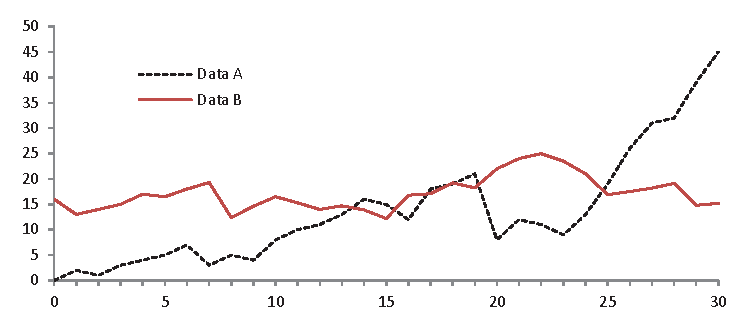
\includegraphics[width=\textwidth]{fig1.eps}
\caption{A figure caption is always placed below the illustration.
Please note that short captions are centered, while long ones are
justified by the macro package automatically.} \label{fig1}
\end{figure}

\begin{theorem}
This is a sample theorem. The run-in heading is set in bold, while
the following text appears in italics. Definitions, lemmas,
propositions, and corollaries are styled the same way.
\end{theorem}


\begin{proof}
Proofs, examples, and remarks have the initial word in italics,
while the following text appears in normal font.
\end{proof}
For citations of references, we prefer the use of square brackets
and consecutive numbers. Citations using labels or the author/year
convention are also acceptable. The following bibliography provides
a sample reference list with entries for journal
articles~\cite{ref_article1}, an LNCS chapter~\cite{ref_lncs1}, a
book~\cite{ref_book1}, proceedings without editors~\cite{ref_proc1},
and a homepage~\cite{ref_url1}. Multiple citations are grouped
\cite{ref_article1,ref_lncs1,ref_book1},
\cite{ref_article1,ref_book1,ref_proc1,ref_url1}.


\begin{thebibliography}{8}
\bibitem{ref_article1}
Author, F.: Article title. Journal \textbf{2}(5), 99--110 (2016)

\bibitem{ref_lncs1}
Author, F., Author, S.: Title of a proceedings paper. In: Editor,
F., Editor, S. (eds.) CONFERENCE 2016, LNCS, vol. 9999, pp. 1--13.
Springer, Heidelberg (2016). \doi{10.10007/1234567890}

\bibitem{ref_book1}
Author, F., Author, S., Author, T.: Book title. 2nd edn. Publisher,
Location (1999)

\bibitem{ref_proc1}
Author, A.-B.: Contribution title. In: 9th International Proceedings
on Proceedings, pp. 1--2. Publisher, Location (2010)

\bibitem{ref_url1}
LNCS Homepage, \url{http://www.springer.com/lncs}. Last accessed 4
Oct 2017
\end{thebibliography}
\end{document}
